% =====================================================================
% 10-minute Beamer slides (+ 10 minutes Q&A with appendix backup slides).
% Build:  pdflatex presentation.tex && pdflatex presentation.tex
% =====================================================================
\documentclass[10pt,aspectratio=169]{beamer}

% ---- Theme --------------------------------------------------------------
\usetheme{Madrid}
\usecolortheme{beaver}
\setbeamertemplate{navigation symbols}{}
\setbeamertemplate{caption}[numbered]
\setbeamerfont{footnote}{size=\tiny}
\setbeamertemplate{frametitle continuation}{}   % suppress "(cont.)"

% ---- Packages -----------------------------------------------------------
\usepackage[T1]{fontenc}
\usepackage{amsmath,amssymb,amsthm}
\usepackage{braket}
\usepackage{graphicx}
\usepackage{stmaryrd}
% \usepackage{pdfpcnotes}
\usepackage{booktabs}
\graphicspath{{./}{../assets/}}

% ---- Metadata -----------------------------------------------------------
\title[Generalised measurement incompatibility]{Quantification of generalised\\
  measurement incompatibility of mutually unbiased bases}
\author[Raul-Andrei Pop]{Raul-Andrei Pop}
\institute[\'Ecole Polytechnique]{%
  \'Ecole Polytechnique \\[0.4em]
  \small Advisors: Marc-Olivier Renou, Lucas-Amadeus Tendick \\
  \small PhIQuS group, Inria Paris-Saclay / LIX}
\date{Lab Research Project, 2025--2026}

% =====================================================================
\begin{document}

% ============================================================
% MAIN DECK -- 10 min, 9 frames
% ============================================================

\begin{frame}[plain]
  \titlepage
  \note{%
    Good [afternoon]. I'm Raul-Andrei Pop, and this is my lab
    research project on the generalised measurement incompatibility of
    mutually unbiased bases, supervised by Marc-Olivier Renou and Lucas
    Tendick in the PhIQuS group.

    \medskip
    The one-line version: I take a known tool for measuring how
    incompatible quantum measurements are, and I extend it to a much
    broader family of compatibility structures.%
  }
\end{frame}

% ============================================================
% INTRO TO QUANTUM MEASUREMENTS + MUBs
% ============================================================

% --- 0a. Projective measurements ----------------------------
\begin{frame}{Quantum states and projective measurements}
  A quantum system is described by a state vector
  $\ket{\psi} \in \mathcal{H}$ -- or, more generally, a density operator
  $\rho \succeq 0$ with $\mathrm{Tr}(\rho) = 1$ -- on a
  finite-dimensional Hilbert space $\mathcal{H} = \mathbb{C}^{d}$.

  \medskip
  \textbf{Projective measurement} on $\mathcal{H}$: a family
  $\{\Pi_a\}_{a = 1}^{n}$ of orthogonal projectors that sum to the identity,
  \[
    \Pi_{a}\Pi_{b} \;=\; \delta_{ab}\,\Pi_{a},
    \qquad \sum_{a} \Pi_{a} \;=\; I.
  \]

  \textbf{Born rule.} The probability of obtaining outcome $a$ on the state $\rho$ is
  \[
    P(a \mid \rho) \;=\; \mathrm{Tr}(\rho\,\Pi_{a}).
  \]

  \medskip
  Outcomes are intrinsically \alert{random}; non-commuting observables cannot be diagonalised in a common basis, hence cannot be read out by a single projective family.
  \note{%
  Quick foundations. A quantum system is a density operator ρ — positive, trace one. The simplest measurement is projective: a set of orthogonal projectors summing to the identity, with outcome probabilities given by the Born rule. The key physical fact I'll build on is at the bottom: non-commuting observables can't be diagonalised together, so no single projective measurement reads them all out at once. That impossibility is exactly what 'incompatibility' will formalise.
  }
\end{frame}

% --- 0b. POVMs ----------------------------------------------
\begin{frame}{POVMs: the most general quantum measurement}
  In practice (noisy detectors, indirect measurements, ancillary systems) one needs measurements that are \alert{not projective}.

  \medskip
  \textbf{POVM} -- \emph{positive operator-valued measure}: a family $\{M_{a}\}_{a = 1}^{n}$ of Hermitian, \alert{positive semidefinite} operators that sum to the identity,
  \[
    M_{a} \;\succeq\; 0,
    \qquad \sum_{a} M_{a} \;=\; I.
  \]
  Born rule extends component-wise: $\;P(a \mid \rho) = \mathrm{Tr}(\rho\,M_{a})$.

  \medskip
  \begin{itemize}
    \item Every projective measurement is a POVM (with $M_{a}^{2} = M_{a}$).
    \item POVMs allow $\mathrm{rank}(M_{a}) > 1$, more outcomes than $\dim \mathcal{H}$, and non-commuting elements.
  %   \item \alert{Naimark's theorem}: every POVM arises as a projective measurement on an enlarged Hilbert space, with the ancilla traced out.
  \end{itemize}

  \medskip
  POVMs are the natural setting for the joint-measurability question studied in this work.
\end{frame}

% --- 1. Motivation (~1 min) ----------------------------------
\begin{frame}{Motivation: incompatibility as a resource}
  \textbf{Classical:} all observables can be measured jointly.\\
  \textbf{Quantum:} some sets of measurements are \alert{incompatible} -- no single experiment reproduces their statistics.

  \medskip
  Incompatibility is a \alert{necessary resource} for
  \begin{itemize}
    \item Bell nonlocality, EPR steering, quantum contextuality
    \item Quantum key distribution, state discrimination, random access codes
  \end{itemize}

  \medskip
  \alert{Mutually unbiased bases (MUBs)} are, in many scenarios, the \emph{maximally incompatible} measurements:
  $\;|\!\braket{b_i | b'_j}\!|^2 = 1/d$ for every pair.

  \medskip
  \begin{block}{In this work}
    We compute the noise robustness of incompatibility for MUBs, and
    extend the framework to \alert{richer compatibility structures}.
  \end{block}
\end{frame}

% --- 2. Setup (~1.5 min) -------------------------------------
\begin{frame}{Setup: joint measurability \& white-noise robustness}
  A family of POVMs $\{M_{a|x}\}$ is \alert{jointly measurable} iff there exists a single parent POVM $\{G_\lambda\}$ and probabilities $p(a\mid x, \lambda)$ with
  \[
    M_{a|x} \;=\; \sum_\lambda p(a\mid x, \lambda)\,G_\lambda.
  \]

  Mix with white noise at level $\eta \in [0, 1]$:
  $\;M_{a|x}^\eta = \eta\,M_{a|x} + (1{-}\eta)\,\mathrm{Tr}(M_{a|x})\,I/d$.

  \medskip
  \begin{block}{Noise-robustness threshold}
    \[
      \eta^{\star} \;=\; \max\bigl\{\,\eta : \{M^\eta_{a|x}\}\text{ is jointly measurable}\,\bigr\}.
    \]
  \end{block}

  $\eta^{\star}$ is computable exactly by a \alert{semidefinite program} (Wolf, P{\'e}rez-Garc{\'i}a, Fern{\'a}ndez, 2009; Designolle \emph{et al.}, PRL 122, 050402, 2019).
\end{frame}

% --- 2b. Why MUBs? -------------------------------------------
\begin{frame}{Why MUBs? -- the most incompatible measurements}
  Two orthonormal bases $\{\ket{b_i}\}, \{\ket{b'_j}\}$ of $\mathbb{C}^{d}$ are
  \alert{mutually unbiased} iff
  \[
    \bigl|\!\braket{b_i | b'_j}\!\bigr|^{2} \;=\; \frac{1}{d}
    \qquad \forall\, i, j,
  \]
  i.e.\ preparing in any state of one basis produces a \emph{uniformly random} outcome in the other.

  \medskip
  \textbf{Why are MUBs the natural target for studying incompatibility?}
  \begin{itemize}
    \item Among all families of $k$ POVMs in dimension $d$, MUBs are conjectured to \alert{minimise} $\eta^{\star}$: they are the families that remain incompatible under the \alert{most} white noise.
    \item Designolle \emph{et al.}\ (2019) derived analytical bounds on $\eta^{\star}$ that are saturated specifically by MUB families in several regimes.
    \item For prime-power $d$, the Wootters--Fields construction (1989) gives an explicit complete set of $d + 1$ MUBs; we work in $d \in \{2, 3, 5, 7, 11\}$.
    \item MUBs also appear in quantum tomography, QKD (e.g.\ BB84), and entropic uncertainty relations.
  \end{itemize}

  \medskip
  \alert{$\Rightarrow$ MUBs are the canonical benchmark family for any new incompatibility scenario.}
\end{frame}

% --- 3. Hypergraphs + our generalisation (~1.5 min) ----------
\begin{frame}{Compatibility hypergraphs (Quintino \emph{et al.}, 2019)}
  For $3$ or more measurements, compatibility can be studied in a more complex way: for example triples can be pairwise compatible yet not jointly measurable as a whole.

  \medskip
  \begin{columns}[T]
    \column{0.50\textwidth}
    We can model a set of measurements as a hypergraph $\mathcal{C} = [C_1, \dots, C_N]$, where each hyperedge lists a subset that must be jointly measurable.

    \medskip
    \alert{Our contribution.} An SDP parameterised by an \emph{arbitrary} hypergraph. Two canonical cases:
    \begin{description}
      \item[\texttt{compatible(k)}] $\mathcal{C} = \{(1,\dots,k)\}$\\
        $\Rightarrow$ full $k$-wise JM.
      \item[\texttt{pair(k)}] $\mathcal{C} = \{(i, j) : i < j\}$\\
        $\Rightarrow$ only jointly measure pairs $(i, j)$
    \end{description}

    \column{0.50\textwidth}
    \centering
    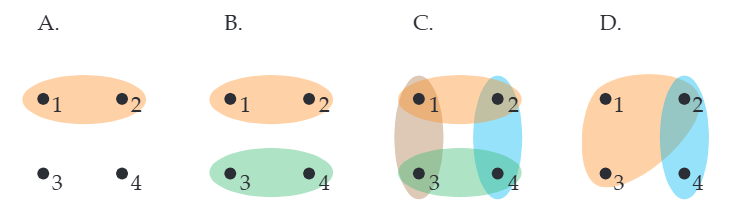
\includegraphics[width=\textwidth]{hypergraphs.png}\\[0.4em]
    \scriptsize Examples on 4 measurements (Fig.~1, arXiv:1902.05841).
  \end{columns}
\end{frame}

% --- 4. Pairwise + analytical bound (~1.5 min) ---------------
\begin{frame}{Pairwise generalization + closed-form lower bound}
  \begin{columns}[T]
    \column{0.55\textwidth}
    \textbf{Geometric picture.} Pairwise-compatible families lie in the convex hull of single-pair JM families. Strictly weaker than full JM.

    \medskip
    \textbf{Equal-weight case:} $p_{ij} = 1/\binom{k}{2}$.
    Branch-counting under MUB symmetry yields:
    \begin{block}{Closed-form bound for pairwise generalization}
      \[
        \eta^{\star}_{(k-1)}(k, d) \;=\;
          1 \;-\; \frac{\sqrt d}{k\,(\sqrt d + 1)}.
      \]
    \end{block}
    \alert{Tight} to solver precision in every case we checked.

    \column{0.45\textwidth}
    \centering
    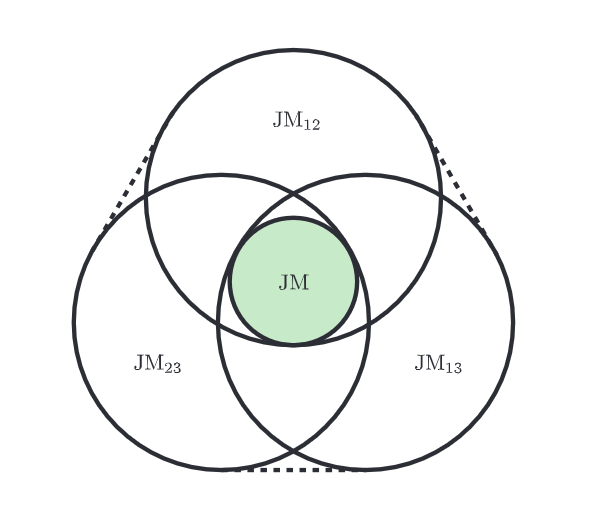
\includegraphics[width=0.90\textwidth]{convex-3-measurements.png}\\[0.4em]
    \scriptsize $JM \subset \mathrm{conv}(JM_{12}, JM_{13}, JM_{23})$.
  \end{columns}
\end{frame}

% --- 5. Numerical results (~2 min) ---------------------------
\begin{frame}{Numerical results}
  \begin{columns}[T]
    \column{0.48\textwidth}
    \centering
    \textbf{Table 1.}\;Full JM (reproduces Designolle et. al., 2019)\\[0.4em]
    \scriptsize
    \begin{tabular}{c|cccc}
      \hline
      $k\,\backslash\,d$ & 2 & 3 & 5 & 7 \\
      \hline
      2 & 0.7071 & 0.6830 & 0.6545 & 0.6371 \\
      3 & 0.5774 & 0.5686 & 0.5393 & 0.5101 \\
      4 & ---    & 0.5000 & 0.4615 & 0.4436 \\
      5 & ---    & ---    & X      & X      \\
      6 & ---    & ---    & 0.4082 & X      \\
      8 & ---    & ---    & ---    & 0.3536 \\
      \hline
    \end{tabular}\\[0.5em]
    \footnotesize Matches closed forms to $10^{-4}$.
    \\``X'' = computationally expensive (~hours for $d^k > 3000$).

    \column{0.52\textwidth}
    \centering
    \textbf{Table 2.}\;All-pairs hypergraph (new)\\[0.4em]
    \scriptsize
    \begin{tabular}{c|ccccc}
      \hline
      $k\,\backslash\,d$ & 2 & 3 & 5 & 7 & 11 \\
      \hline
      2 & 0.7071 & 0.6830 & 0.6545 & 0.6371 & 0.6158 \\
      3 & 0.8047 & 0.7887 & 0.7697 & 0.7581 & 0.7439 \\
      4 & ---    & 0.8415 & 0.8273 & 0.8186 & 0.8079 \\
      5 & ---    & ---    & 0.8618 & 0.8549 & 0.8463 \\
      6 & ---    & ---    & 0.8848 & 0.8791 & 0.8719 \\
      7 & ---    & ---    & ---    & 0.8963 & 0.8902 \\
      8 & ---    & ---    & ---    & 0.9093 & 0.9040 \\
      9 & ---    & ---    & ---    & ---    & 0.9146 \\
      \hline
    \end{tabular}\\[0.5em]
    \footnotesize Every entry matches the analytical bound\\
    $\Rightarrow$ \alert{tightness} of the equal-weight mixture.
  \end{columns}
\end{frame}

% --- 6. Qualitative observation (~1 min) -----------------------------------
\begin{frame}{Qualitative observation: robustness increases with $k$ in the pairwise case}
  \centering
  \medskip
  \begin{tabular}{lcc}
    \toprule
    & \textbf{Full JM} & \textbf{Pairwise Generalization} \\
    & $\eta^{\star}_{\text{JM}}(k, d)$ & $\eta^{\star}_{(k-1)}(k, d)$ \\
    \midrule
    Behaviour in $k$  & \alert{decreasing} & \alert{increasing} \\
    Limit as $k \to \infty$ & $\to 0$ & $\to 1$ \\
    Limit as $d \to \infty$ & $\to 0$ & $\to 1 - 1/k$ \\
    \bottomrule
  \end{tabular}

  \bigskip
  \begin{itemize}
    \item In the pairwise SDP, a fixed measurement appears in only $k{-}1$ of the $\binom{k}{2}$ branches -- a vanishing fraction $2/k$. Its "responsibility" dilutes as $k$ grows.
    \item Explicit instance of the Quintino et al. hierarchy: finer hypergraphs $\Rightarrow$ looser constraint $\Rightarrow$ larger $\eta^{\star}$.
  \end{itemize}
\end{frame}

% --- 7. Conclusion + outlook (~1 min) ------------------------
\begin{frame}{Summary and outlook}
  \textbf{Contributions.}
  \begin{enumerate}
    \item Reproduced the standard JM noise-robustness SDP for MUBs in prime dimensions $d \in \{2, 3, 5, 7\}$.
    \item Generalised the program to \alert{arbitrary compatibility hypergraphs}.
    \item Produced numerical results for the all-pairs hypergraph
    \item Derived the \alert{closed-form bound}
          $\eta^{\star} = 1 - \sqrt d / [\,k(\sqrt d + 1)\,]$
          for the generalized pairwise incompatibility, numerically tight in every case.
  \end{enumerate}

  \bigskip
  \textbf{Three natural extensions.}
  \begin{description}
    \item[(i)] \emph{Dual SDP} $\Rightarrow$ analytical proof of tightness.
    \item[(ii)] \emph{Intermediate hypergraphs} (triples, $(k\!-\!2)$-subsets).
    \item[(iii)] \emph{Composite dimensions} ($d = 6$: open MUB problem).
  \end{description}
\end{frame}

% --- 8. Thank you --------------------------------------------
\begin{frame}[plain]
  \vfill
  \centering
  {\Huge \textbf{Thank you!}}\\[1.5em]
  
\end{frame}

% =====================================================================
% APPENDIX -- backup slides for Q&A (not in TOC)
% =====================================================================
\appendix

\begin{frame}[plain]
  \centering
  \vfill
  {\LARGE \textbf{Questions}}\\[1em]
  
  \vfill
\end{frame}

% --- BACKUP A: the qubit SDP ----------------------------------
\begin{frame}{Questions -- the qubit SDP, explicitly}
  Pauli observables and their eigenprojectors:
  \[
    \sigma_X = \begin{pmatrix} 0 & 1 \\ 1 & 0 \end{pmatrix}, \;\;
    \sigma_Z = \begin{pmatrix} 1 & 0 \\ 0 & -1 \end{pmatrix}, \;\;
    \Pi^{(X)}_{\pm} = \tfrac{1}{2}(I \pm \sigma_X), \;\;
    \Pi^{(Z)}_{\pm} = \tfrac{1}{2}(I \pm \sigma_Z).
  \]
  Noisy POVM elements $M^{\eta}_{a|x} = \eta\,\Pi^{(x)}_a + (1-\eta)\,I/2$:
  \[
  \footnotesize
  M^{\eta}_{+|X} = \tfrac{1}{2}\!\begin{pmatrix} 1 & \eta \\ \eta & 1 \end{pmatrix},\;
  M^{\eta}_{-|X} = \tfrac{1}{2}\!\begin{pmatrix} 1 & -\eta \\ -\eta & 1 \end{pmatrix},\;
  M^{\eta}_{+|Z} = \tfrac{1}{2}\!\begin{pmatrix} 1{+}\eta & 0 \\ 0 & 1{-}\eta \end{pmatrix},\;
  M^{\eta}_{-|Z} = \tfrac{1}{2}\!\begin{pmatrix} 1{-}\eta & 0 \\ 0 & 1{+}\eta \end{pmatrix}.
  \]
  Find $G_{\lambda_X \lambda_Z} \in \mathbb{C}^{2 \times 2}$ Hermitian:
  \[
  \begin{aligned}
    \text{maximise} \quad & \eta \in [0, 1] \\
    \text{s.t.} \quad     & G_{\lambda_X \lambda_Z} \succeq 0,
                            \;
                            {\textstyle\sum_{\lambda_X, \lambda_Z}}
                            G_{\lambda_X \lambda_Z} = I, \;
                            {\textstyle\sum_{\lambda_Z}}
                            G_{a\, \lambda_Z} = M^{\eta}_{a|X}, \;
                            {\textstyle\sum_{\lambda_X}}
                            G_{\lambda_X\, a} = M^{\eta}_{a|Z}.
  \end{aligned}
  \]
  \begin{block}{Optimal value}
    $\eta^{\star}(2, 2) = 1/\sqrt 2 \approx 0.7071$ — matches our $(k, d) = (2, 2)$ entry.
  \end{block}
\end{frame}

% --- Questions B: the general k-MUB SDP --------------------------
\begin{frame}{Questions -- the general $k$-MUB joint-measurability SDP}
  For $k$ noisy MUBs in dimension $d$, with $m = d$ outcomes per setting:
  \[
  \begin{aligned}
    \text{maximise} \quad & \eta \in [0, 1] \\
    \text{s.t.} \quad     & G_{\lambda_1 \cdots \lambda_k} \succeq 0
                            \quad \forall (\lambda_1, \dots, \lambda_k) \in \llbracket 1, m \rrbracket^k, \\
                          & \textstyle\sum_{\lambda_1, \dots, \lambda_k} G_{\lambda_1 \cdots \lambda_k} = I, \\
                          & \textstyle\sum_{\lambda : \lambda_j = a} G_{\lambda_1 \cdots \lambda_k}
                            = M^{\eta}_{a | j}
                            \quad \forall j \in \llbracket 1, k \rrbracket,\ \forall a \in \llbracket 1, m \rrbracket.
  \end{aligned}
  \]
  Variable count: $d^{k}$ Hermitian $d \times d$ matrices -- \alert{exponential in $k$}.
\end{frame}

% --- Questions C: scaling comparison -----------------------------
\begin{frame}{Questions -- why pairwise scales well but full JM does not}
  Per-cell SDP variable count:
  \medskip
  \centering
  \begin{tabular}{c|rr|r}
    \toprule
    $(k, d)$ & full JM $d^{k}$ & all-pairs $\binom{k}{2}(d^2 + (k-2)d)$ & ratio \\
    \midrule
    $(4, 5)$ & 625              & 210                                    & 3$\times$ \\
    $(4, 7)$ & 2{,}401          & 378                                    & 6$\times$ \\
    $(5, 7)$ & 16{,}807         & 630                                    & 27$\times$ \\
    $(6, 7)$ & 117{,}649        & 945                                    & 124$\times$ \\
    $(8, 7)$ & \alert{5{,}764{,}801} & 2{,}548                            & 2{,}262$\times$ \\
    \bottomrule
  \end{tabular}

  \bigskip
  Full JM: \alert{$\mathcal{O}(d^k)$} (exponential).
  \quad Pairwise: \alert{$\mathcal{O}(k^3 d^2)$} (polynomial).

  \medskip
  \footnotesize
  \textbf{Why hours?}
  Each interior-point iteration costs $\mathcal{O}(d^k \cdot d^3) \approx 2 \cdot 10^9$
  operations just for the per-block eigendecompositions, with hundreds of iterations to
  converge -- plus a multi-GB memory footprint that defeats cache. CVXPY
  canonicalisation alone takes tens of minutes at this size.

  \medskip
  \normalsize
  Hence Table 1 has many empty cells; Table 2 is complete.
\end{frame}

% --- Questions D: derivation of the analytical bound -------------
\begin{frame}{Questions -- derivation of the closed-form bound}
  Equal-weight case $p_{ij} = 1 / \binom{k}{2}$. By MUB symmetry, every setting $x$ is presented in $k-1$ \emph{active} branches at noise $\eta^{\star}(2, d)$ and in $\binom{k}{2} - (k-1)$ \emph{inactive} branches at noise $1$.

  \medskip
  Affineness of $\eta \mapsto M^{\eta}$:
  \[
    \eta_{\text{eff}}
    \;=\; \tfrac{1}{\binom{k}{2}}
          \bigl[\,(k-1)\,\eta^{\star}(2, d)
                 + \tfrac{(k-1)(k-2)}{2}\,\bigr]
    \;=\; \tfrac{1}{k}\bigl[\,2\,\eta^{\star}(2, d) + k - 2\,\bigr].
  \]

  \medskip
  Substituting $\eta^{\star}(2, d) = (2 + \sqrt d)/[\,2(\sqrt d + 1)\,]$ (Designolle):
  \[
    \eta_{\text{eff}}
    \;=\; 1 + \tfrac{1}{k}\Bigl(\tfrac{2 + \sqrt d}{\sqrt d + 1} - 2\Bigr)
    \;=\; 1 - \tfrac{\sqrt d}{k\,(\sqrt d + 1)}.
  \]

  \medskip
  Boundary check: $k = 2$ recovers $\eta^{\star}(2, d) = (2 + \sqrt d)/[\,2(\sqrt d + 1)\,].\;\checkmark$
\end{frame}

% --- Questions E: implementation notes ---------------------------
\begin{frame}{Questions -- implementation \& code}
  All SDPs formulated with \alert{CVXPY} (Python).
  \begin{itemize}
    \item Solver: \textsc{Clarabel} for small cases ($d^k \le 100$), \textsc{Scs} for the rest ($\epsilon = 10^{-7}$, $10^{5}$ iterations).
    \item Cap: $d^k > 3000$ omitted in Table 1; no cap for Table 2 (polynomial scaling).
    \item Every closed-form entry of \cite{Designolle2019} reproduced to $10^{-4}$; solver status \texttt{optimal} in every reported cell.
  \end{itemize}

  \medskip
  Core routines (\texttt{compatibility\_hypergraph.py}):
  \begin{itemize}
    \item \texttt{robustness\_hypergraph(M, hypergraph)} -- the generalised SDP driver.
    \item \texttt{hypergraph\_compatible(k)} -- $\{(1, \dots, k)\}$ for full JM.
    \item \texttt{hypergraph\_pair(k)} -- $\{(i, j) : i < j\}$ for pairwise generalization.
  \end{itemize}
\end{frame}

\end{document}
